\section{Implementation}
\label{sec:implementation}
We will have a look at the implementation of the engine and the development framework in this section. Since there is much focus on performance, this section may be characterized by its performance discussions. We will also see how a model (or two) can be implemented within this framework.


\subsection{About Ngene}
\emph{Ngene} is a flexible, generic, multi-purpose genetic algorithm engine written in C++ with heavy emphasis on performance and flexibility. The engine is divided into logical modules that can easily be interchanged or extended upon in order to fit the intended purpose. A sub-goal of this engine is also portability. Anybody should be able to use this engine on their platform of choice, regardless of whether they are sitting on Microsoft\textregistered Windows\texttrademark or Unix, and hardware based on Intel\textregistered Architecture or Power Architecture.

The prototype for this engine started out as an assignment for a sub-symbolic artificial intelligence course. It was written in Python, which later proved to be too slow for this kind of application, and later partially ported to C++ because I wanted to learn the language at the time. The project got lost in a pile of other assignments and was never heard from again. The engine was finally picked up again, re-designed and completed for the purpose of this thesis.

\subsubsection{Modular Design}
The modular design of Ngene is the heart of it all. In order to achieve maximum flexibility, the engine should be able to change any of its parts without having to do anything special. Should the user feel like changing the mutation method, this should be as easy as changing a single line in a configuration file. This is most useful because different experiments may require different genotypes or any other modules. With that in mind, the design is therefore broken into the following logical modules:

\begin{itemize}
	\itemsep=0pt
	\item\textbf{Core} - The genetic algorithm itself
	\item\textbf{Fitness} - Assesses the fitness of a genotype
	\item\textbf{Genotype} - Generates the genotype and translates them to phenotype
	\item\textbf{Mating} - Crosses two genotypes
	\item\textbf{Mutator} - Mutates a genotype
	\item\textbf{Selector} - Randomly selects a genotype
\end{itemize}

Each of these modules are like the parts of a car. Roulette selection can be exchanged for tournament selection, just like how the motor can be exchanged for another to enhance its performance. Of course, without the technical difficulties involved when changing a car engine. This modular design will allow users to swap a module without prior knowledge of programming. In fact, writing code will not be needed at all unless a new module is required. This design will also keep the code much cleaner and easier to maintain.

\subsubsection{Why C++?}
In a sense, one can say that this project was made possible because of my prototype in Python. It taught me many higher level concepts that is practically non-existant in lower level languages such as C++. Without it, I probably wouldn't have been able to bring the project to the level it is today. Especially without the concept of a dynamic type, the idea of a container that can contain anything from an integer, to a string, to a floating type number, I would still have trouble trying to compensate for it with complex algorithms to deal with raw data pointers. Most importantly, it taught me the importance of optimization and use of libraries.

Choosing a programming language depends on what kind of application you want to write. A simple program with no special requirements can be written in any language. For instance, a mail client written in Python will perform equally well as any other client because the focus lies on fetching and displaying e-mails and the ability to manage them in an easy way. The features are more important than the extra two milliseconds it takes to perform a query. However, there are applications for which performance is more important than anything. Arguably, such programs should be written in one of two ways: In assembly (or machine code) or C/C+. While assembly is rarely used these days due to being practically unreadable for mortals, C and C++ is often used for time critical applications. Unlike languages that depend on a virtual machine (C\#, Java), or an interpreter (some LISP dialects, Python), code written in C/C++ is compiled directly to machine code before executed, often yielding much better performance.

C++ is thought of as being a middle level language. It has the advantages of both the lower (machine code) and higher level languages, but also the inherent disadvantages. For example, all memory management must be explicitly handled in the code. C++ does not have a garbage collector typically found in higher level languages. This means that we have to be extra careful of deallocating memory to avoid leaks, and prevent access of invalid memory addresses. Furthermore, C++ doesn't come with as big a convenience library as those found in aforementioned languages. Such libraries save a lot of time, eliminating rewriting often used algorithms and the headache of debugging faulty code. Fortunately, efforts are being made to ease the implementation through external libraries.

\subsubsection{Boost C++ Libraries}
\emph{Boost}\footnote{\url{http://www.boost.org/}} is a collection of libraries which complement the C++ Standard Library (STL). Ngene makes use of this collection, saving time and effort, and guaranteeing that such code works as it should.

\paragraph{\textbf{Boost.Any}}\cite{henney2001}
A problem with writing a generic genetic algorithm in a strongly typed programming language, is that different studies require different data types to be passed around the system. CGP, for instance, uses integers to implement its genotype, while ArtDev3D uses a custom defined type. In other models, there may even be a mix of different types. It is impossible to foresee what may or may not be used, and we are thus forced to abstract this away. Unfortunately, C++ will not allow an integer variable to store any other data type than an integer. In a higher level language like Python, there exists a container that can store any type of data:

\begin{verbatim}
>>> foo = 1 + 2
>>> print foo
3
>>> foo = "awesome"
>>> print foo
awesome
>>> _
\end{verbatim}

Doing something similar in C++ would simply give us a syntax error. To make such a container in C++, will require some coding. Fortunately, this has already been implemented and is freely available as part of \emph{Boost}. The modular design would otherwise not work without it, at least not within given time constraint. The container, called \emph{Boost.Any}, does not differ much from the one found in Python and comes only at the cheap cost of requiring a type-casting before the data can be handled as normal.

\paragraph{\textbf{Boost Random Number Library}}\cite{maurer2000}
Another problem with genetic algorithms and development in general is implementing a good pseudo-random number generator. Ngene uses the implementation of \emph{Mersenne twister} pseudo-random number generator also found in the Boost libraries. This generator was chosen for its long period ($2^{19937}-1$ or approximately $4.3*10^{6001}$), and because it is relatively fast compared to other algorithms. It also passes a number of tests for randomness, including Diehard\footnote{A collection of tests to measure the quality of the randomness of the generator, developed by George Marsaglia.} and most of the stricter TestU01 Crush\footnote{Another collection of tests, developed by Pierre L'Ecuyer and Richard Simard.} randomness tests.

\subsubsection{Brief System Overview}
\begin{figure}[!ht]
	\centering
	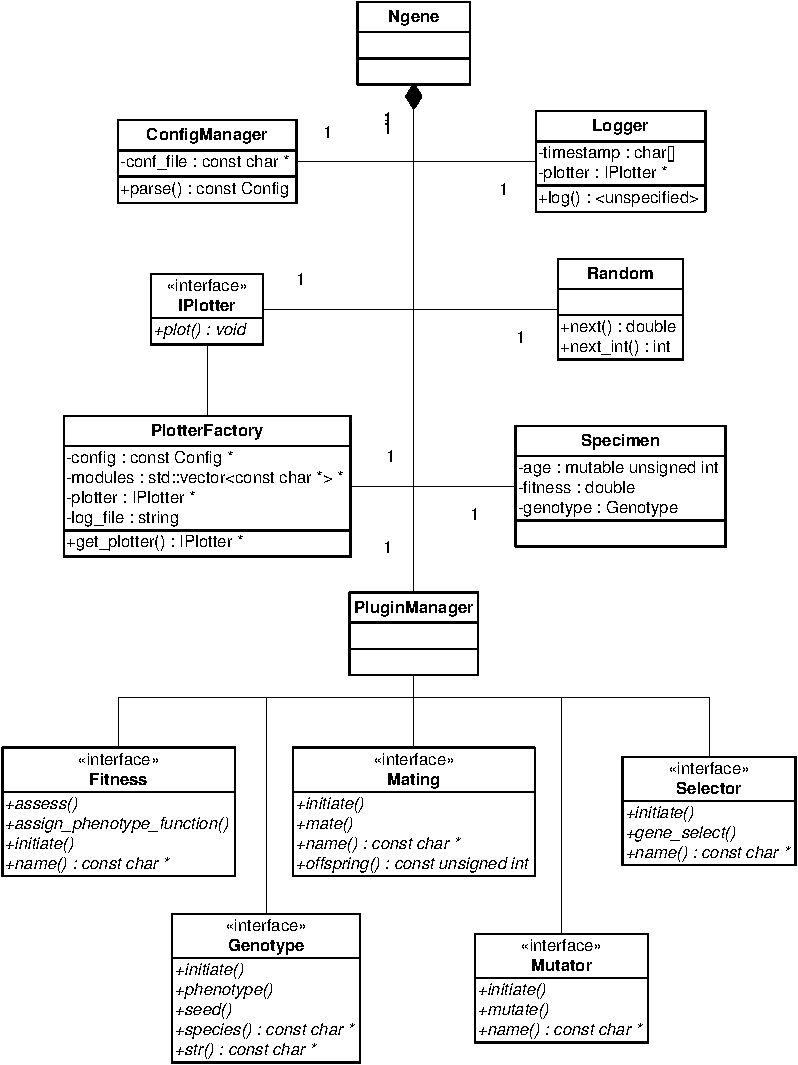
\includegraphics{diagram_ngene}
	\caption{Overview of Ngene}
	\label{fig:diagram_ngene}
\end{figure}

Figure~\ref{fig:diagram_ngene} shows a brief overview of how Ngene is put together. At startup, three of these parts are responsible for what must take place before anything can be run in accordance with the user's parameters. \texttt{ConfigManager} takes care of reading the configuration file and creating a settings object that every other parts have access to. Once the configuration file has been parsed, \texttt{PluginManager} will use this object to find out which modules it's going load. If the user specified tournament selector, it will load the tournament module and make it ready for the genetic engine. When every module is loaded, \texttt{Logger} will use the same settings object to find out how it should log the current run, whether it should plot a fitness/generation graph or just print out the progress on the screen. By now, the genetic algorithm will start. It is a very simple algorithm:

\begin{enumerate}
	\itemsep=0pt
	\item An initial population is randomly generated.
	\item \texttt{Specimen}s are randomly selected for crossover.
	\item Repeat step 2 until the offspring population is of satisfactory size.
	\item Replace adult population with offspring population.
	\item Repeat process from step 2 until the maximum number of generations is reached, or a perfect \texttt{Specimen} is found.
	\item Write log/graph and final \texttt{Specimen} to disk.
\end{enumerate}

The final step is the responsibility of \texttt{Logger}. \texttt{Logger} has no knowledge of what format the \texttt{Specimen} should be written as. Be it a text file, an image or a proprietary format, it will simply request the \texttt{Genotype} module to give it some data to write to disk. The output format is actually coded in each \texttt{Genotype} module because it rarely changes for a single experiment and/or model. Otherwise, a new module must be written anyway.

\texttt{PluginManager}, along with the responsibilities of loading and releasing modules, will also act as a layer between the modules and the genetic engine itself. The engine will never have to bother with the specifics of each module. It should be able to just tell what a module ought to do. Of course, this requires that the modules implement a predefined interface in order to be compatible with this layer. These are described in more detail in the system documentation for Ngene.


\subsection{Ngene Development Framework}
\begin{figure}[!ht]
	\centering
	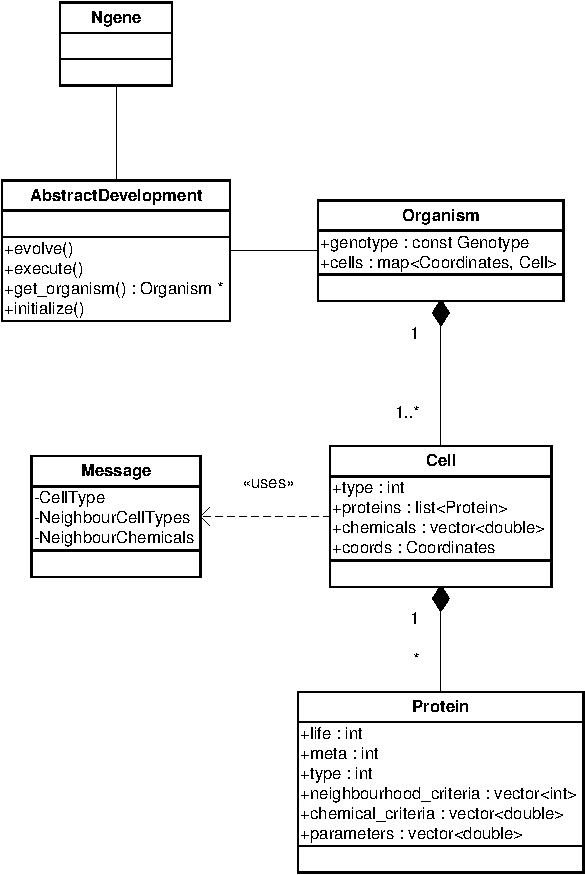
\includegraphics{diagram_ndevframe}
	\caption{Overview of Ngene Development Framework}
	\label{fig:diagram_ndevframe}
\end{figure}

The downside of having such a flexible design, is that users are given too much freedom in implementing their own modules, making it difficult to compare two models without having to factor in differences in implementations. A common generic development framework can eliminate these factors and ease the implementation at the same time. The Ngene Development Framework is an attempt of such a framework.

The framework provides a code base that implements a common development algorithms, along with common concepts such as a cell and protein (see fig.~\ref{fig:diagram_ndevframe}). More importantly, it also includes an intercellular communication (see fig.~\ref{fig:diagram_ndevframe_msg}) algorithm. As we saw earlier with ArtDev3D and CGP, the communication between the two differs a lot. It is important that the message system can provide what is needed for both systems and still be able to clearly distinguish the differences so that we can easily take this into consideration when comparing the two models. Use of this code base is enforced in order to ensure that all comparison made between different development models are based on a common ground.

\begin{figure}[!ht]
	\centering
	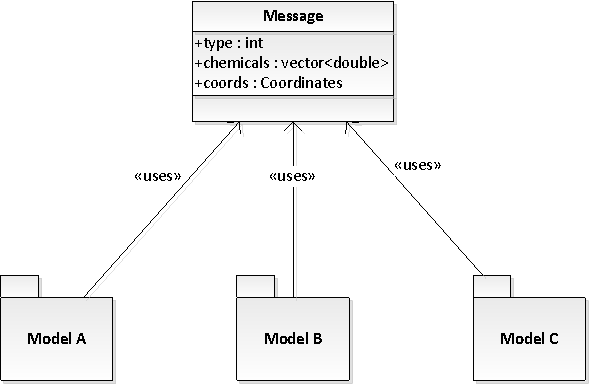
\includegraphics{diagram_ndevframe_msg}
	\caption{A common message implementation should let users easier distinguish the differences in intercellular communication between different models.}
	\label{fig:diagram_ndevframe_msg}
\end{figure}

Figure~\ref{fig:diagram_ndevframe_common-base} should demonstrate this requirement. We can see right away that all three models differ because model A and B use chemicals, while C uses proteins. We also see that model B and C require a control program in addition to their cell programs. When models are implemented using the framework, we will be able to clearly see which parts a model uses and why it is unique compared to another model. Since a common code base is used, you can rule out the possibility that the development or genetic algorithm may differ.

\begin{figure}[!ht]
	\centering
	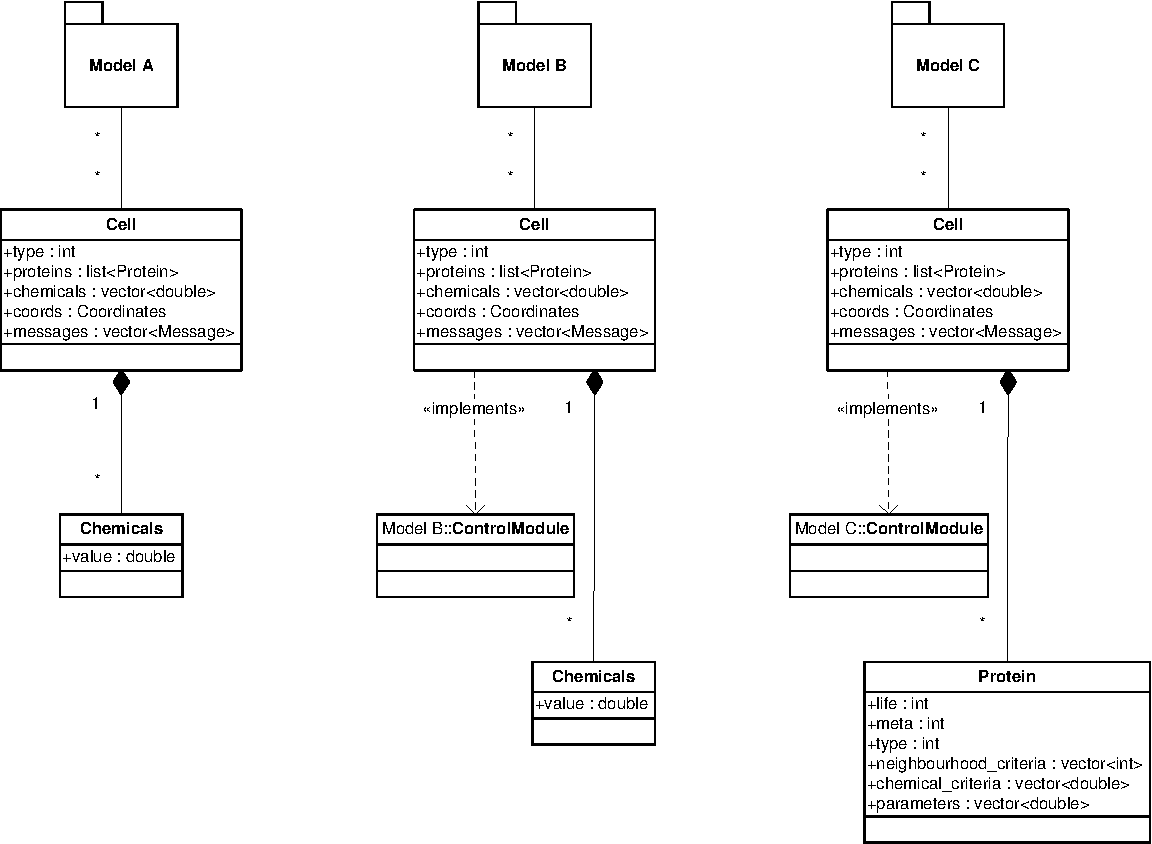
\includegraphics[scale=0.8]{diagram_ndevframe_common-base}
	\caption{Albeit different, all three models still use the same implementation of a cell, chemicals and proteins, and receive the same messages.}
	\label{fig:diagram_ndevframe_common-base}
\end{figure}

Since the framework is going to be used by many users, speed is also a concern when designing it. It is important that the framework is not only flexible and easy to use, but also perform relatively well compared to other implementations. Lots of thought as been put into how to represent the organisms themselves. In the current implementation, a C++ Standard Library (STL) \texttt{<map>} is used to store the cells using their coordinates as the key value. Other alternatives were also considered:

\begin{center}
	\begin{tabular}{ r | c | c | c }
		~ & STL \texttt{<map>} & STL \texttt{<vector>} & STL \texttt{<ext/hash\_map>} \\
		\hline
		element access & $O(log~n)$ & $O(1)$ & $O(1)$ \\
		\hline
		insertion & $O(log~n)$ & $O(1)$ & $O(1)$ \\
		\hline
		search & $O(log~n)$ & $O(n)$ & $O(1)$ \\
	\end{tabular}
	\label{tbl:speed}
\end{center}

A quick glance at the comparison table and the \texttt{<ext/hash\_map>} may seem like the best choice to go with. However, there are some drawbacks that must be taken into consideration.

A hash table creates a unique key based on a number of properties found in the value to be stored. The key is used to retrieve the value at some later point. The hashing algorithm is essential in both that it determines how uniform the distribution will be over the array, and how well the hash table will perform overall. A too simple hashing algorithm will often experience collisions, i.e. a lot of values will have the same key. When this occurs, there are several ways to handle it (also called collision resolution). In worst case scenario, the key will point to a list, thus making the hash table perform like a linked list. Insertion is still constant but lookup may be as bad as $O(n)$. On the other hand, an overly complex hashing algorithm will also deteriorate performance because more CPU cycles is spent calculating a good hash value. Regardless of how good the hashing algorithm is, collisions will always occur. The \emph{birthday paradox} predicts that it doesn't take many elements before the chance of a collision exceeds 95\%, even for very big arrays. It is clear that the hash table cannot guarantee its performance advantage over the other containers. Besides, for the experiments conducted in this thesis, the number of cells rarely exceeded 1000. If we use a \texttt{<map>}, which is the case here, it will take at most ten comparisons to find an element by its key value. A good hashing algorithm will use approximately the same number of operations to calculate a key value, perform lookup, and resolve any collisions.

The problem with \texttt{<vector>} is that it is one-dimensional. This makes it difficult to efficiently calculate x, y and z values of a coordinate since we don't know how many cells there will be. Another drawback is that it will take $O(n)$ time to look for neighbours. This can be worked around by maintaining an up to date neighbours list for every cell. This will make lookup $O(1)$ but increase insertion time to $O(n)$. \texttt{<map>} offers easier facilities to perform such tasks more efficiently. Later, in chapter \ref{sec:improvements}, we will discuss a custom implementation that will theoretically perform better than mentioned containers.


\subsubsection{Using the Framework}
\begin{figure}[!ht]
	\centering
	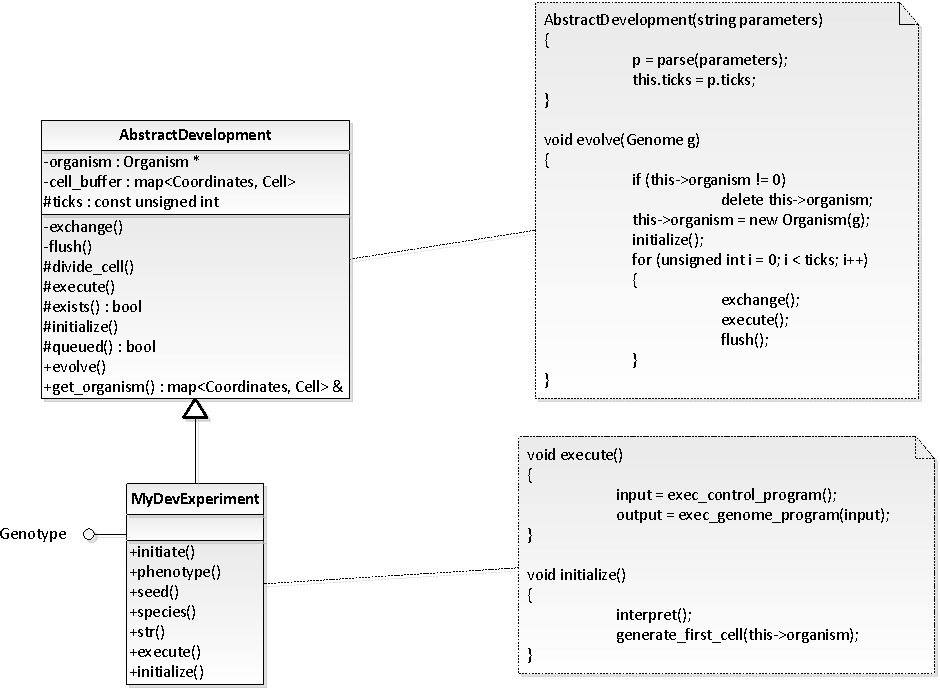
\includegraphics{diagram_ndevframe_ex}
	\caption{An example of how one can implement \texttt{MyDevExperiment}.}
	\label{fig:diagram_ndevframe_ex}
\end{figure}

The framework was designed to ease the implementation effort as much as possible. The whole code base can be inherited from \texttt{AbstractDevelopment} (see fig.~\ref{fig:diagram_ndevframe_ex}). To port a model to this framework, only two functions need to be implemented: \texttt{execute()} and \texttt{initialize()}. The latter is executed once with every new organism that is to be developed, and can be used to unpacking the genotype to a cellular program and/or generating initial cells in the organism. The \texttt{execute()} function is called every development step/tick, for every cell in the organism. Here, the cell program from the genotype can be executed as well as any control programs that might be needed. Note that any messages sent has already been received and are stored in the cells themselves by the time a cell is given the chance to fulfil its purpose in a tick. It will not be possible to actually access the organism itself from this function in order to avoid accidental tampering.

For the purpose of this thesis, two models were implemented within this framework not only to test the flexibility and performance of this framework but also to see what is missing and what areas need improvement.


\subsubsection{ArtDev3D}
\label{sec:Implementation:ArtDev3D}
Porting Johan H{\o}ye's master's thesis\cite{hoye2006} to Ngene's framework has been a matter of finding out what occurs in a cell during a development step, and whether or not there are external processes that needs to be accounted for. As described in chapter~\ref{sec:Models:ArtDev3D}, the genotype of the model does not do all the work in a cell. The cell has its own control program as well. The program can be summarized as the following steps:

\begin{enumerate}
	\itemsep=0pt
	\item Clear all queued actions.
	\item For every active protein, queue their action requests.
	\item Accumulate actions (add them together to execute in one go).
	\item Execute action \#1: Transcribe proteins.
	\item Execute action \#2: Regulate chemical levels.
	\item Execute action \#3: Perform cell division.
	\item Execute action \#4: Change cell type.
	\item Remove dead proteins.
\end{enumerate}

The implementation of the model might seem overwhelming at first impression. There is a heavy use of biological concepts in the code and the simplest operation may span across many classes, and files, as a result. This alone makes it hard to follow the code flow, but the little system documentation that does exist, fortunately, does provide with some help though it consists mainly of commentaries in the source files themselves. While his efforts in making it understandable are much appreciated, it might be beneficial to flatten the structure a bit and get rid of some of the redundant structures that are inspired by nature. There is another reason for why this was altered as well.

In theory, such an implementation can have a negative impact on performance. When a simple operation performed must call a function to call another function to call yet another function and so on, can put the calling stack under strain. This may occur because this does not happen only once, but several times every development step in a single cell. And as we know, there are plenty of cells in an organism. Flattening the structure as mentioned, will reduce the number of calls and potentially improve performance.

There was also an issue that was identified and patched in the port. In most models, cells are developed simultaneously. In order to achieve this, information must be exchanged between all cells before a cell can execute its functions. This is to ensure that the cell program will execute based on the current state of the organism without interfering for other cells. In ArtDev3D, this is not properly implemented. Upon execution, the cell will start collecting requests from its proteins. The proteins can request an action when they are activated, i.e. when the state of the cell and its neighbours are above a threshold. The requests are queued up and then executed. The problem with this, is that it all happens in a single step. Thus, cells that already have had their turn before the current cell, will have an altered state. Actions are therefore based on a mix of ``newer'' information from these cells, and ``old'' information from the rest. When porting this code to the new framework, the cell will no longer have direct access to other cells. Instead, it will receive messages from (or a snapshot of) nearby cells before the development step takes place in any cell. This change may alter the outcome of the model, but was addressed merely out of necessity. We cannot have two different development algorithms as that would defeat the very purpose of the framework.


\subsubsection{Cartesian}
\label{sec:cartesian}
This model was implemented from scratch with help from Dr. Julian F. Miller himself. The model is rather simple because the whole cell program is in the genotype. The implementation should only need to translate the genotype into a working digital circuit and be able to ``run'' it.

The genotype is an array of integers. The number of integers depend on the number of layers and how many nodes each layer consists of. The number of layers and nodes per layer is static. This will keep it simple, and also make the crossover less complicated. As far as I know, this should be in line with Dr. Miller's implementation as well. Each node consists of four integers - three that will serve as connection points to other nodes while the last one will point to a specific function. The function will get its input from the connected nodes' output. The functions implemented here are basic boolean operations, in addition to the four elementary mathematical operations.

\begin{itemize}
	\itemsep=0pt
	\item \texttt{AND}, \texttt{MUX}, \texttt{NAND}, \texttt{NOR}, \texttt{OR}, \texttt{XNOR}, \texttt{XOR}
	\item addition, division, multiplication, subtraction
\end{itemize}

Upon initialization, the engine will receive the genotype and will start translating it into a digital circuit. The cell program is then executed:

\begin{itemize}
	\item An input bitstring is generated from the chemical levels and types of the current cell together with its neighbours.
	\item The bitstring is sent to the cell program.
	\item The output bitstring is parsed. Some bits will give the cell a new type, the rest will tell the cell to divide in particular directions and how much chemicals these will receive.
	\item Chemical diffusion according to $(c_{ij})_{new} = \frac{1}{2}(c_{ij})_{old} + \frac{1}{16}\sum_{k, l \in N} (c_{kl})_{old}$
\end{itemize}

Dr. Miller has also provided with important information regarding his implementation of the model. His implementation actually contains a bug that causes the program to only read the most significant bit from the chemical bits in the neighbours. The other bits are set to zero. When he later identified and patched this bug, he found that the bug was actually beneficial to the model. This bug was also re-implemented in order to make it closer to the original implementation.
